\graphicspath{{images/act_1.3/}}
\subsection{Inverse kinematics approach}
\label{subsec:inverse_kinematics_approach}
The objective of this activity is to control movement of the ur5 robot end-effector so that it follows the Cartesian sinusoidal reference trajectory of activity \ref{subsec:generate_sinusoidal_reference}. The simulation starts with initial joint configuration $\mathbf{q_0}=\begin{bmatrix} 0.0 & -1.0 & 1.0 & 0.5 & 0.0 & 0.5 \end{bmatrix}$ rad and end-effector $\mathbf{p_0}=\begin{bmatrix}  0.577 &   0.192 &   0.364 \end{bmatrix}$~m. Likewise, the Cartesian sinusoidal reference trajectory starts at $\mathbf{p_0}$. Then, inverse kinematics computes joint reference points ($\mathbf{q_{des}}$) from the Cartesian sinusoidal trajectory ($\mathbf{p_{des}}$); Algorithm \ref{lst:inverse_kinematics} describes a function to perform inverse kinematics using jacobian damped pseudo-inverse. Finally, movement of the ur5 robot is controlled with a proportional-derivative control method, at joint level, with feed-forward terms. Thus, control law can be computed as 
\begin{equation}
	\boldsymbol{\tau}
	=\mathbf{M}\mathbf{\ddot{q}_{des}} + \mathbf{K_p e} + \mathbf{K_d \dot{e}},
	\label{eq:articular_PD}
\end{equation}
\noindent where $\mathbf{M}$ represent inertia matrix, $\mathbf{{q}_{des}}$ is desired joint trajectory, $\mathbf{e}=\mathbf{q_{des} - q}$ is position error, and $\mathbf{K_p, K_d}$ are the proportional and derivative gains respectively. \vspace{.5cm}

\begin{lstlisting}[language=Python,caption={Function to compute inverse kinematics with jacobian damped psedo-inverse method.}, label={lst:inverse_kinematics}]
def inverse_kinematics_position(self, x_des, q0):
    """
    @info: computes inverse kinematics with jacobian damped pseudo-inverse.

    @inputs:
    -------
        - xdes  :   desired position vector
        - q0    :   initial joint configuration (it's very important)
    @outputs:
    --------        
        - q_best  : joint position
    """         
    best_norm_e     = 1e-6 
    max_iter        = 10
    delta           = 1
    lambda_         = 0.0000001
    q               = copy(q0)

    for i in range(max_iter):
        p, _ = self.forward_kinematics(q) # current position
        e   = x_des - p      # position error
        J   = self.jacobian(q)[0:3, 0:self.ndof] # position jacobian [3x6]
        J_damped_inv =  self.jacobian_damped_pinv(J, lambda_) # inverse jacobian [6x3]
        dq  = np.dot(J_damped_inv, e)
        q   = q + delta*dq
                   
        # evaluate convergence criterion
        if (np.linalg.norm(e)<best_norm_e):
            best_norm_e = np.linalg.norm(e)
            q_best = copy(q) 
    return q_best 
\end{lstlisting}

The Algorithm \ref{lst:articular_PD} control the movements of ur5 robot end-effector to track the Cartesian sinusoidal reference trajectory of activity~\ref{subsec:generate_sinusoidal_reference}. In this file, the articular PD control method is configured with ${K_{p}}=600$ $\mathrm{\frac{N.m}{rad}}$ and $K_{d}= 30$ $\mathrm{\frac{N.m.s}{rad}}$. On one hand, Figure \ref{fig:act_1.3_ee_position} shows that trajectory tracking performance at the Cartesian space is poor with mean norm error at each axis ($||e_x||, ||e_y||, ||e_z||$) of ($0.0811$, $0.0176$, $0.062$) cm respectively. The constant position error in $z$-axis could be reduced by adding gravity terms on control law \eqref{eq:articular_PD}. On the other hand, Figure \ref{fig:act_1.3_joint_position} shows that trajectory tracking performance at joint space is poor because there are position error in all joints. The constant joint position error could be reduced by adding gravity terms on control law \eqref{eq:articular_PD}.

\begin{lstlisting}[language=Python,caption={Move the ur5 robot end-effector using a articular proportional-derivative control method, \eqref{eq:articular_PD}, and inverse kinematics, Algorithm \ref{lst:inverse_kinematics}, to compute joint reference points from Cartesian sinusoidal reference trajectory of activity \ref{subsec:generate_sinusoidal_reference}.}, label={lst:articular_PD}]
# =========================
#   Configuration of node
# =========================
# create a node: 
rospy.init_node("inverse_kinematics_approach")
# public in topic /joint_states	to send joint data	
pub = rospy.Publisher('joint_states', JointState, queue_size=1000)
# loop rate (in Hz)
rate 	= rospy.Rate(1000)		# 1000 [Hz]
dt 		= 1e-3					# 1  [ms]
# object(message) type JointState
jstate = JointState()

# ==========================================
#   Set initial joint configuration of UR5
# ==========================================
# initial configuration: position, velocity and acceleration 
q0 =   np.array([ 0.0, -1.0, 1.0, 0.5, 0.0, 0.5])
dq0 =  np.array([0.0, 0.0, 0.0, 0.0, 0.0, 0.0]) 
ddq0 = np.array([0.0, 0.0, 0.0, 0.0, 0.0, 0.0]) 

# desired trajectory: position, velocity and acceleration
q_des =   np.array([ 0.0, -1.0, 1.0, 0.5, 0.0, 0.5])
dq_des =  np.array([0.0, 0.0, 0.0, 0.0, 0.0, 0.0]) 
ddq_des = np.array([0.0, 0.0, 0.0, 0.0, 0.0, 0.0]) 

# measured trajectory: position, velocity and acceleration
q_med =   np.array([ 0.0, -1.0, 1.0, 0.5, 0.0, 0.5])
dq_med =  np.array([0.0, 0.0, 0.0, 0.0, 0.0, 0.0]) 
ddq_med = np.array([0.0, 0.0, 0.0, 0.0, 0.0, 0.0]) 

# ===========================
#   UR5 robot configuration
# ===========================
# joints name of UR5 robot
jnames = ['shoulder_pan_joint', 'shoulder_lift_joint', 'elbow_joint','wrist_1_joint', 'wrist_2_joint', 'wrist_3_joint']
# path of labs_ur5.urdf
urdf_path = os.path.join(pwd, "../../ur5_description/urdf/labs_ur5.urdf")
# the class robot load labs_ur5.urdf
ur5_robot = Robot(q0, dq0, dt, urdf_path)
# number of degress of freedom
ndof = ur5_robot.ndof

# create inertia matrix 
M = np.zeros([ndof,ndof])
# create nonlinear effects vector
b = np.zeros(ndof)
# create gravity vector
g = np.zeros(ndof)

# ==============================================
#   set initial cartesian configuration of UR5
# ==============================================
# initial cartesian configuration: position, velocity and acceleration
p0 = ur5_robot.get_ee_position()
dp0 = np.array([0.0, 0.0, 0.0])
ddp0 = np.array([0.0, 0.0, 0.0])

# desired cartesian trajectory: position, velocity and acceleration
p_des = copy(p0)
dp_des = np.array([0.0, 0.0, 0.0])
ddp_des = np.array([0.0, 0.0, 0.0])

# measured cartesian trajectory: position, velocity and acceleration
p_med = copy(p0)
dp_med = np.array([0.0, 0.0, 0.0])
ddp_med = np.array([0.0, 0.0, 0.0])

# ===============================
#   PD controller configuration
# ===============================
# proportional gain
kp = 600*np.ones(ndof)
# derivative gain
kd = 30*np.ones(ndof)
# control vector
tau = np.zeros(ndof)    

#===============
#   Simulation
#===============
t = 0.0             # [sec] 
sim_duration = 5.0  # [sec]
sine_duration = 4.0    # [sec]

while not rospy.is_shutdown():
    # desired cartesian trajectory
    p_des[0], dp_des[0], ddp_des[0] = sinusoidal_reference_generator(p0[0], 0.1, 1.5, sine_duration, t)

    # jacobian: position xyz [3x6]
    J = ur5_robot.jacobian(q_des)[0:3, 0:6] 
    # jacobian: dampend pseudo-inverse [6x3] 
    J_pinv = ur5_robot.jacobian_damped_pinv(J)
    # jacobian: time derivative [3x6]
    dJ = ur5_robot.jacobian_time_derivative(q_des, dq_des)[0:3, 0:6]
    
    # desired joint trajectory
    q_des = ur5_robot.inverse_kinematics_position(p_des, q_des)
    dq_des = np.dot(J_pinv, p_des)
    ddq_des = np.dot(J_pinv, ddp_des - np.dot(dJ, dq_des))

    # error: position and velocity
    e 	=  q_des - q_med
    de 	=  dq_des - dq_med    

    # compute inertia matrix
    M = ur5_robot.get_M()

    # control law: PD + feed-forward term
    tau_ff = M.dot(ddq_des)
    tau = tau_ff + np.multiply(kp, e) + np.multiply(kd, de)
    
    # send control signal
    ur5_robot.send_control_command(tau)
    # update states
    q_med, dq_med, ddq_med = ur5_robot.read_joint_position_velocity_acceleration()
    p_med, dp_med, ddp_med = ur5_robot.read_cartesian_position_velocity_acceleration()

    # publish message
    jstate.header.stamp = rospy.Time.now()
    jstate.name 		= jnames			# Joints position name
    jstate.position 	= q_med
    jstate.velocity 	= dq_med
    pub.publish(jstate)

    # update time
    t = t + dt
    
    # stop simulation
    if t>=sim_duration:
        print("stopping rviz ...")
        break
    rate.sleep()
\end{lstlisting}

\vspace*{0cm}
\begin{figure}
	\centering
	\subfloat[]{
	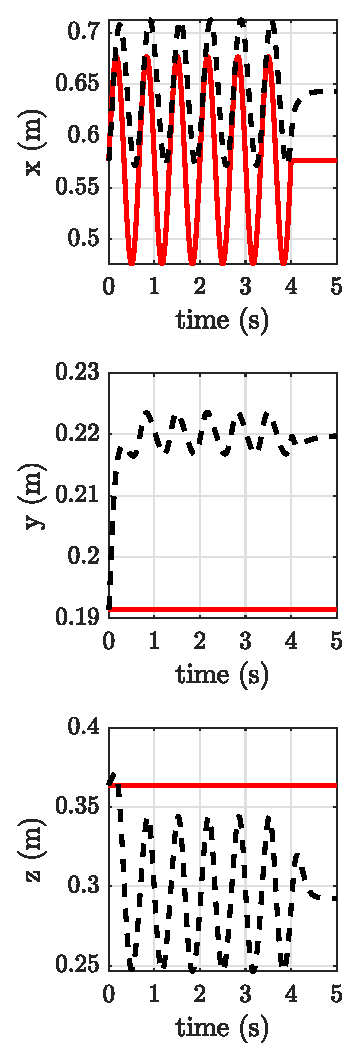
\includegraphics{ee_position.eps}
	}
	\hfill
	\subfloat[]{
	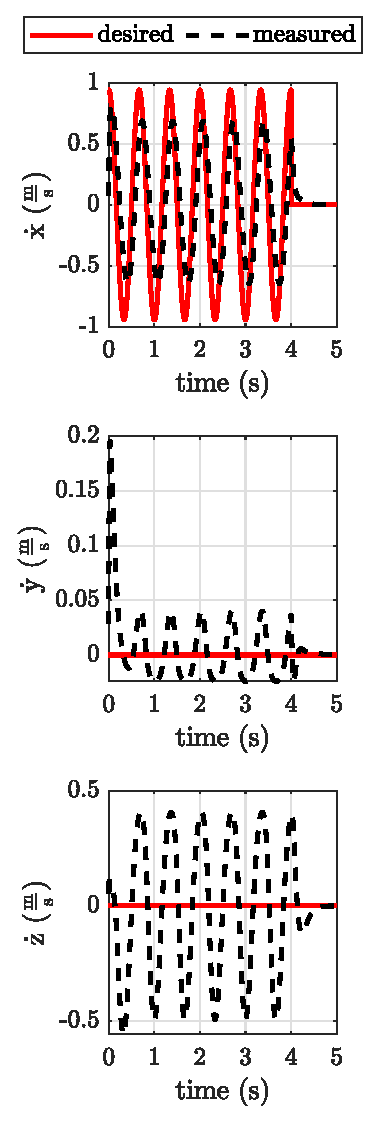
\includegraphics{ee_velocity.eps}
	}	
	\hfill
	\subfloat[]{
	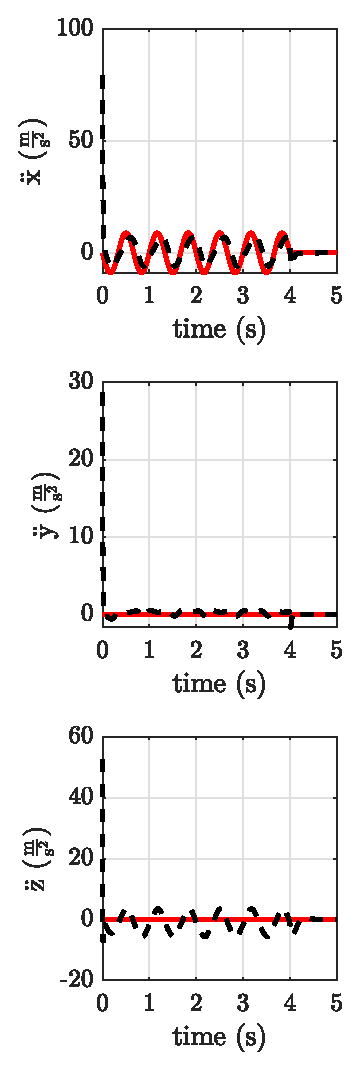
\includegraphics{ee_acceleration.eps}
	}		
	\caption{Cartesian trajectory tracking performances using  articular proportional-derivative control method, \eqref{eq:articular_PD}, with  ${K_{p}}=600$ $\mathrm{\frac{N.m}{rad}}$ and $K_{d}= 30$ $\mathrm{\frac{N.m.s}{rad}}$: (a) position, (b) velocity and (c) acceleration.}
	\label{fig:act_1.3_ee_position}
\end{figure}

\begin{figure}
    \centering
    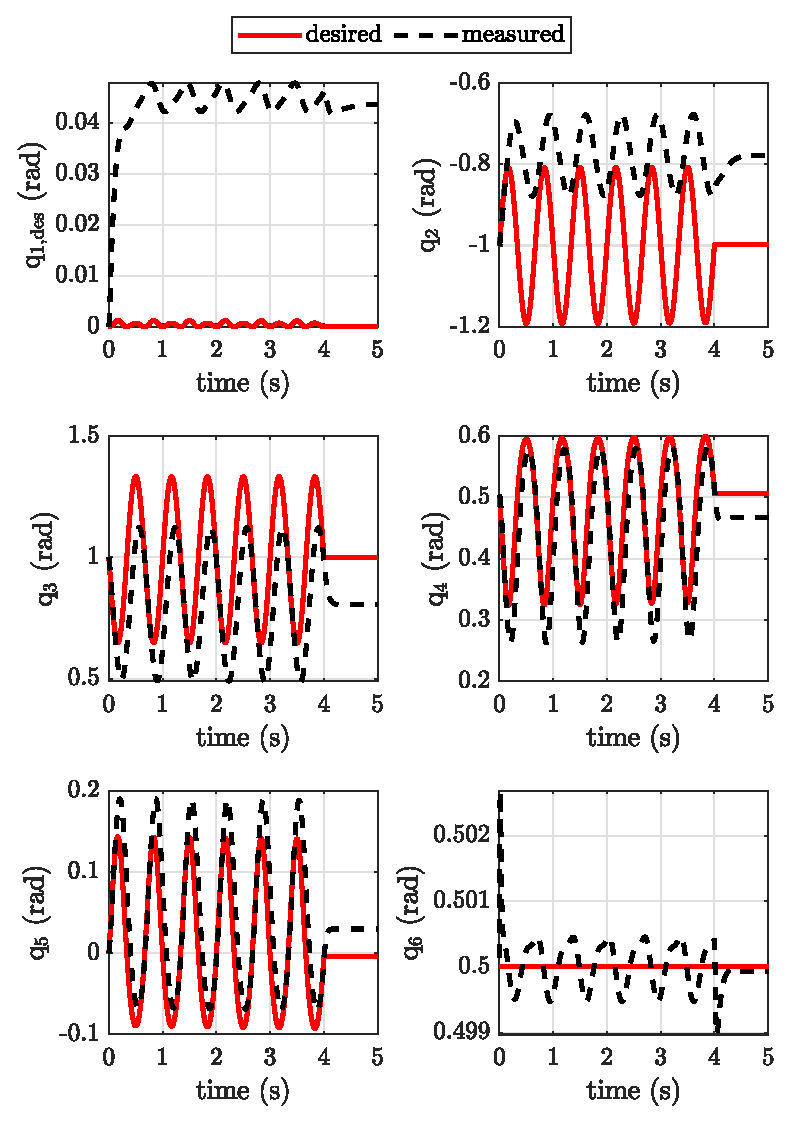
\includegraphics{joint_position.eps}
    \caption{Angular trajectory tracking performances using articular proportional-derivative control method, \eqref{eq:articular_PD}, with  ${K_{p}}=600$ $\mathrm{\frac{N.m}{rad}}$ and $K_{d}= 30$ $\mathrm{\frac{N.m.s}{rad}}$.}
    \label{fig:act_1.3_joint_position}
\end{figure}
